\documentclass[11pt,a4paper]{article}

% ================================================================
% Adaptive Frames for Hybrid Intelligence
% Overleaf-compatible manuscript (compile with pdfLaTeX + BibTeX)
% ================================================================

\usepackage[a4paper,top=2.0cm,bottom=2.1cm,left=2.15cm,right=2.15cm]{geometry}
\usepackage[T1]{fontenc}
\usepackage[utf8]{inputenc}
% Latin Modern is included in standard TeX/Overleaf installations and keeps
% the project portable. Replace with newtxtext,newtxmath if preferred.
\usepackage{lmodern}
\usepackage{microtype}
\usepackage{xcolor}
\usepackage{graphicx}
\usepackage{booktabs}
\usepackage{tabularx}
\usepackage{array}
\usepackage{multirow}
\usepackage{amsmath,amssymb,mathtools}
\usepackage{enumitem}
\usepackage[most]{tcolorbox}
\usepackage{tikz}
\usetikzlibrary{arrows.meta,positioning,fit,calc,shapes.geometric,backgrounds}
\usepackage{listings}
\usepackage{caption}
\usepackage{subcaption}
\usepackage{natbib}
\usepackage[hidelinks]{hyperref}
\usepackage[nameinlink,noabbrev]{cleveref}
\usepackage{fancyhdr}
\usepackage{titlesec}

% ---------- ARU-inspired palette ----------
\definecolor{ARUNavy}{HTML}{123B5D}
\definecolor{ARURed}{HTML}{C81D3C}
\definecolor{ARUGold}{HTML}{C8A45D}
\definecolor{ARUBlueGrey}{HTML}{DCE5EA}
\definecolor{ARUCream}{HTML}{F7F2E8}
\definecolor{ARUPink}{HTML}{F4DDE3}
\definecolor{Ink}{HTML}{202A33}
\definecolor{SoftGrey}{HTML}{F3F5F6}
\definecolor{Green}{HTML}{28856B}

\hypersetup{
  colorlinks=true,
  linkcolor=ARUNavy,
  citecolor=ARURed,
  urlcolor=ARUNavy,
  pdftitle={Adaptive Frames for Hybrid Intelligence},
  pdfauthor={Kirti Prakash}
}

\titleformat{\section}{\Large\bfseries\color{ARUNavy}}{\thesection}{0.7em}{}
\titleformat{\subsection}{\large\bfseries\color{ARUNavy}}{\thesubsection}{0.7em}{}
\titleformat{\subsubsection}{\normalsize\bfseries\color{Ink}}{\thesubsubsection}{0.7em}{}
\titlespacing*{\section}{0pt}{1.5em}{0.6em}

\pagestyle{fancy}
\setlength{\headheight}{22pt}
\fancyhf{}
\fancyhead[L]{\small\color{ARUNavy}Adaptive Frames for Hybrid Intelligence}
\fancyhead[R]{\small\color{ARUNavy}Prakash}
\fancyfoot[C]{\small\thepage}
\renewcommand{\headrulewidth}{0.4pt}
\renewcommand{\headrule}{\hbox to\headwidth{\color{ARURed}\leaders\hrule height \headrulewidth\hfill}}

\setlist[itemize]{leftmargin=1.35em,itemsep=2pt,topsep=3pt}
\setlist[enumerate]{leftmargin=1.55em,itemsep=2pt,topsep=3pt}
\renewcommand{\arraystretch}{1.18}
\newcolumntype{Y}{>{\raggedright\arraybackslash}X}

\newtcolorbox{takehome}[1][]{
  enhanced,breakable,colback=ARUNavy,colframe=ARUNavy,
  coltext=white,boxrule=0pt,arc=1.5mm,
  borderline west={3pt}{0pt}{ARUGold},
  fonttitle=\bfseries,title={Take-home message},#1}

\newtcolorbox{criticalbox}[1][]{
  enhanced,breakable,colback=ARUCream,colframe=ARUGold,
  coltitle=ARUNavy,fonttitle=\bfseries,title={Critical point},#1}

\newtcolorbox{examplebox}[1][]{
  enhanced,breakable,colback=SoftGrey,colframe=ARUBlueGrey,
  coltitle=ARUNavy,fonttitle=\bfseries,title={Worked example},#1}

\lstdefinestyle{pythonstyle}{
  language=Python,
  basicstyle=\ttfamily\footnotesize,
  keywordstyle=\color{ARURed}\bfseries,
  commentstyle=\color{Green},
  stringstyle=\color{ARUNavy},
  backgroundcolor=\color{SoftGrey},
  frame=single,
  rulecolor=\color{ARUBlueGrey},
  breaklines=true,
  showstringspaces=false,
  columns=fullflexible,
  xleftmargin=0.4em,
  framexleftmargin=0.3em
}

\newcommand{\Frame}{\mathcal{F}}
\newcommand{\Frames}{\mathbb{F}}
\newcommand{\Obs}{\mathcal{O}}
\newcommand{\Goals}{\mathcal{G}}
\newcommand{\Repair}{\mathcal{R}}
\newcommand{\Risk}{\operatorname{Risk}}
\newcommand{\Cost}{\operatorname{Cost}}
\newcommand{\Violation}{\operatorname{Violation}}
\newcommand{\Fit}{\operatorname{Fit}}

\begin{document}
\hypersetup{pageanchor=false}

\begin{titlepage}
  \pagecolor{ARUCream}
  \begin{tikzpicture}[remember picture,overlay]
    \fill[ARURed] (current page.north west) rectangle ([yshift=-7pt]current page.north east);
    \fill[ARUNavy] (current page.south west) rectangle ([yshift=1.7cm]current page.south east);
    \fill[ARUGold] ([xshift=1.4cm,yshift=1.7cm]current page.south west) rectangle
      ([xshift=1.75cm,yshift=2.0cm]current page.south west);
  \end{tikzpicture}
  \vspace*{1.4cm}
  {\color{ARURed}\bfseries\large PERSPECTIVE AND REFERENCE ARCHITECTURE}\par
  \vspace{0.55cm}
  {\color{ARUNavy}\fontsize{28}{33}\selectfont\bfseries
  Adaptive Frames for Hybrid Intelligence\par}
  \vspace{0.35cm}
  {\color{Ink}\Large From Minsky's Knowledge Structures to
  Grounded, Probabilistic and Governed AI Agents\par}
  \vspace{1.1cm}

  \begin{tcolorbox}[colback=white,colframe=ARUBlueGrey,arc=2mm,boxrule=0.8pt]
  \textbf{Central proposal.} A computational frame should combine an ontology,
  validation constraints, uncertain expectations, active questions, executable
  procedures, transformations, provenance and repair operations. Neural models
  propose; semantic structures define; constraints verify; agents act; evidence
  and provenance determine whether the frame should be retained or revised.
  \end{tcolorbox}

  \vfill
  {\large\bfseries Kirti Prakash}\par
  \vspace{0.15cm}
  {\normalsize Anglia Ruskin University and China Jiliang University teaching programme}\par
  \vspace{0.15cm}
  {\normalsize Semantic Data Technologies}\par
  \vspace{0.55cm}
  {\small Manuscript and executable teaching simulation, 2026}\par
  \vspace{1.2cm}
\end{titlepage}
\nopagecolor
\hypersetup{pageanchor=true}
\pagenumbering{roman}

\begin{abstract}
Marvin Minsky's 1974 frame proposal argued that intelligence depends on
retrieving and adapting large knowledge structures for stereotyped situations.
Frames contain slots, constraints, defaults, procedural attachments,
transformations and links to alternatives. The proposal anticipated contextual
knowledge representation, script-like event models, active information seeking,
explanation by expectation failure and the integration of declarative knowledge
with control. It nevertheless remained an informal research programme: it did
not supply a precise semantics, a scalable frame-selection algorithm, calibrated
uncertainty, a learning procedure, data provenance or empirical evaluation.

This paper develops a contemporary successor: the \emph{adaptive frame}, a
goal-conditioned and temporally situated structure that joins RDF/OWL semantics,
SHACL validation, probabilistic expectations, neural representations,
retrieval-augmented generation, tool-using agents and provenance-aware repair.
We define a formal frame tuple, derive a constrained frame-selection objective,
describe a complete frame lifecycle and propose an evaluation protocol comparing
language-model-only, ontology-only, retrieval-augmented and hybrid systems. A
reproducible Google Colab simulation instantiates the architecture in a movie
knowledge graph. It demonstrates competing frame hypotheses, SPARQL retrieval,
SHACL validation, active questioning, human-confirmed repair, provenance capture
and before/after quality visualisation. The resulting framework converts
Minsky's enduring cognitive insight into an implementable and falsifiable
research programme for trustworthy hybrid intelligence over the next decade.
\end{abstract}

\noindent\textbf{Keywords:} frames; knowledge graphs; semantic web;
neuro-symbolic AI; SHACL; RDF; OWL; retrieval-augmented generation; agents;
provenance; knowledge repair.

\begin{takehome}
The paper's central claim is not that ontologies should replace neural models,
or that language models should replace explicit knowledge. Intelligence requires
a controlled cycle in which learned models propose contextual interpretations,
semantic structures make their commitments explicit, constraints identify
failure, tools obtain missing evidence and provenance-aware repair improves the
system without silently rewriting history.
\end{takehome}

\tableofcontents
\newpage
\pagenumbering{arabic}

% ================================================================
\section{Introduction}
% ================================================================

Artificial intelligence has repeatedly moved between two poles. Symbolic
systems represent concepts and rules explicitly, permitting inspection and
deduction, but often fail when the world is noisy, incomplete or unfamiliar.
Statistical systems learn patterns from data and generalise across surface
variation, but may produce answers that are unsupported, inconsistent or
difficult to update. Foundation models intensify rather than remove this
tension: their linguistic competence is broad, yet factual provenance,
calibration, persistent identity and reliable constraint following remain
open challenges \citep{bommasani2021opportunities,ji2023hallucination}.

Minsky's \emph{A Framework for Representing Knowledge} was an early attempt to
escape this binary \citep{minsky1975framework}. A frame is a remembered
structure for a familiar situation. It contains terminals to be filled,
conditions on possible values, defaults for incomplete observations, procedures
for acquiring or checking values, and connections to alternative frames. A
frame-system links multiple descriptions of the same entity or event, such as
different visual viewpoints. Failure is not merely a negative outcome: a
mismatch helps determine which alternative should be attempted next.

The proposal is often remembered as a precursor to object-oriented records or
ontological classes. That interpretation is too narrow. A Minsky frame combines
at least five functions that modern computing typically separates:

\begin{enumerate}
  \item a \textbf{schema} describing entities and relations;
  \item an \textbf{expectation model} containing typical or default values;
  \item a \textbf{question generator} directing attention to missing evidence;
  \item a \textbf{controller} specifying procedures that may be executed; and
  \item a \textbf{repair mechanism} for explaining and responding to mismatch.
\end{enumerate}

The central research question of this paper is therefore:

\begin{quote}
\emph{How can Minsky's contextual and procedural account of frames be converted
into a formal, learnable, provenance-aware and empirically testable architecture
using contemporary semantic data technologies and foundation models?}
\end{quote}

The paper makes four contributions. First, it critically reconstructs the
original frame proposal, separating its enduring insights from its unresolved
assumptions. Second, it defines an adaptive-frame formalism that distinguishes
hard constraints, soft expectations, defaults, provenance, tools and governance.
Third, it presents a reference architecture grounded in RDF, OWL, SPARQL, SHACL,
vector retrieval and agent actions. Fourth, it specifies a reproducible
simulation and benchmark protocol through which the framework can be falsified,
rather than remaining a conceptual metaphor.

% ================================================================
\section{Minsky's Frame Programme Reconstructed}
% ================================================================

\subsection{Frames as large-grained knowledge structures}

Minsky's initial complaint was representational granularity. Many early vision
and problem-solving systems represented small facts or local features but lacked
larger structures that could organise them. A frame supplies a global hypothesis:
``this is a room'', ``this is a birthday party'', or ``this is a transaction''.
Observations are interpreted relative to the activated hypothesis, and the
hypothesis specifies which observations matter.

This is not equivalent to forcing every observation into a rigid template.
Frames can contain unfilled terminals, weak defaults and alternative branches.
The frame reduces search by making some questions more relevant than others.
Its value therefore lies as much in selective attention as in storage.

\subsection{Terminals, markers and defaults}

A terminal is a position that may be assigned a value. A room frame might
contain terminals for walls, doors, windows, furniture and viewpoint. Terminal
markers constrain what can fill a position. Some terminals refer to lower-level
subframes, enabling hierarchical decomposition.

When observation does not provide a value, a default can be assigned. Defaults
make efficient interpretation possible because most everyday situations are
only partly observed. They also create epistemic risk. A typical value can be
mistaken for a fact, and a historically common value can encode an unjustified
social norm. The original proposal recognises that defaults may be displaced,
but does not specify their confidence, provenance or legitimate scope.

\subsection{Frame-systems and transformations}

Related frames form systems. In the cube example, different views share
terminals representing stable properties while viewpoint transformations alter
the visible configuration. This anticipates multi-view representation: one
entity may have visual, functional, causal, social and regulatory descriptions.
No single description is sufficient for all goals.

The transformation idea is powerful but incomplete. A link labelled
``move right'' or ``later'' does not by itself explain the mechanism, temporal
conditions or causal intervention. A modern version requires explicit event
identity, time, persistence and action-conditioned transition models.

\subsection{Language, discourse and scenarios}

Minsky treats sentence interpretation as partial frame construction. Surface
syntax activates semantic structures; successive sentences contribute to larger
scene, thematic and narrative frames. Familiar scenarios create expectations
about roles and event order. This is close to later script-based accounts
\citep{schank1977scripts} and remains relevant to event extraction and narrative
reasoning.

Crucially, an incomplete frame becomes a collection of questions. If an event
frame expects an agent, object and destination, missing terminals specify what
the system should seek next. Understanding is thus active: the representation
controls information acquisition.

\subsection{Memory, similarity and explanation}

Memory retrieval is presented as problem solving, not as lookup. A cue activates
candidate structures; partial matching preserves valuable assignments; mismatch
may be explained by occlusion, damage, functional substitution or an exceptional
context. Similarity networks connect frames through labelled differences,
anticipating both knowledge-graph neighbourhoods and learned embedding spaces.

Minsky's notion of an ``excuse'' is especially important. It is a structured
explanation of why an expected feature is absent. Modern systems usually return
a score or error label. A frame system should instead distinguish at least four
possibilities: the observation is wrong, the selected frame is wrong, the case
is a legitimate exception, or the representation is inadequate.

\subsection{Control and procedural attachment}

Frames are packets of data and processes. Activated frames establish local
working environments in which procedures can inspect slots, obtain evidence and
trigger alternatives. This avoids both extremes of a single central controller
and completely independent local processes.

The idea prefigures tool-using agents, but it also creates a design hazard. If
knowledge, inference and action are not cleanly separated, a corrupted assertion
may trigger an unsafe operation. Contemporary implementations therefore need
permission boundaries, audit trails and explicit distinctions between proposing,
validating and executing an action.

% ================================================================
\section{Critical Assessment}
% ================================================================

\subsection{What the paper got right}

\begin{table}[ht]
\centering
\caption{Enduring contributions of the frame programme.}
\label{tab:enduring}
\begin{tabularx}{\textwidth}{p{0.22\textwidth}YY}
\toprule
\textbf{Contribution} & \textbf{Why it matters} & \textbf{Contemporary analogue} \\
\midrule
Contextual interpretation & Facts acquire relevance within goals and situations & Contextual retrieval and task-specific subgraphs \\
Defeasible defaults & Systems can operate under incomplete information & Priors, default rules and calibrated prediction \\
Multiple representations & One object supports several valid descriptions & Ontology modules, embeddings and multimodal views \\
Active questions & Missing slots direct information gathering & Active learning, agents and competency questions \\
Mismatch diagnosis & Failure supplies information about representation & SHACL reports, anomaly detection and model criticism \\
Procedural knowledge & Representation is connected to use and action & Tool calling, workflows and policy engines \\
Repair through experience & Learning modifies the representation, not only parameters & Knowledge-graph completion and ontology evolution \\
\bottomrule
\end{tabularx}
\end{table}

These insights challenge a persistent assumption: that intelligence can be
reduced either to deduction over a fixed vocabulary or prediction from a fixed
data distribution. Minsky instead treats representation as provisional,
goal-sensitive and revisable.

\subsection{Where the theory remains incomplete}

\subsubsection{Informal semantics}

The original paper does not define when two frames are equivalent, when a slot
assignment is licensed, or how conflicts between defaults should be resolved.
Without model-theoretic or operational semantics, correctness depends on the
implementer's intuition.

\subsubsection{The selection circularity}

A frame helps interpret observations after it has been selected, but selecting
the correct frame appears to require an interpretation. Similarity and
expectation can generate candidates, yet the theory lacks a principled ranking
and rejection rule. Contemporary dense retrieval can narrow the candidate set,
but semantic and empirical verification are still required.

\subsubsection{Missing learning algorithm}

Learning is described as debugging frames, but the theory does not determine
when to add a slot, introduce an exception, split a frame, merge frames or
forget outdated knowledge. These operations have different consequences and
require evidence thresholds and governance.

\subsubsection{Uncalibrated defaults}

``Weak assignment'' is not a quantitative uncertainty model. Probability,
confidence, source reliability, constraint satisfaction and decision risk are
distinct variables. Collapsing them into a single score recreates the problem
Minsky identified: a number cannot preserve all the considerations that formed
it.

\subsubsection{Underdeveloped temporality and causality}

Before-and-after frames encode succession but not necessarily causation. A
modern account must represent events, timestamps, interventions, persistence,
counterfactual alternatives and versioned beliefs. Otherwise, the system may
mistake correlation or temporal order for a causal mechanism
\citep{pearl2009causality}.

\subsubsection{No empirical test}

The memo offers illustrations but no benchmark, baseline, complexity analysis,
ablation or user study. Its explanatory reach is consequently greater than its
demonstrated computational performance.

\subsection{The critique of logic reconsidered}

Minsky rightly objects to unrestricted classical deduction as a complete model
of intelligence. Classical logic provides no native preference for relevant
premises, treats conclusions monotonically and handles everyday exceptions
poorly. Nevertheless, later description logics, default logics,
truth-maintenance systems, probabilistic logics and paraconsistent approaches
address important parts of this criticism \citep{brachman1977structural,
reiter1980logic,dekleer1986atms}.

The productive conclusion is not ``logic failed''. It is that logic should be
assigned a bounded role. Formal semantics can define identities and necessary
relationships; shapes can validate operational requirements; probabilistic
models can rank plausible interpretations; and agents can obtain additional
evidence.

% ================================================================
\section{From Frames to Semantic and Neuro-Symbolic Systems}
% ================================================================

\subsection{RDF and OWL as the semantic substrate}

RDF represents knowledge as subject--predicate--object triples
\citep{rdf2014concepts}. OWL adds formally interpreted classes, properties,
individuals and restrictions \citep{owl2012overview}. These technologies supply
globally identifiable terms, interoperable graphs and machine-processable
semantics. They provide part of a frame---principally its declarative schema---
but not its full behaviour.

Under the open-world assumption, the absence of a triple does not entail that
the corresponding statement is false. An OWL reasoner may therefore infer new
class memberships without treating a missing release year as a data error. That
distinction is essential: logical inference and operational completeness are
different tasks.

\subsection{SHACL as explicit verification}

SHACL defines shapes against which RDF graphs can be validated
\citep{shacl2017}. A shape can state that a movie requires exactly one title,
that a duration is an integer within a range, or that a value belongs to an
allowed set. A validation report identifies focus nodes, failed paths,
severities and messages. This resembles Minsky's frame verification, but SHACL
does not determine whether the data or the shape should be repaired.

\subsection{Retrieval, embeddings and foundation models}

Knowledge-graph embeddings and graph neural networks provide graded similarity
over entities and relations \citep{nickel2016review,hamilton2017representation}.
Retrieval-augmented generation combines parametric models with external memory,
improving updateability and evidence access \citep{lewis2020rag}. Graph-based
retrieval can additionally organise entity communities and global themes
\citep{edge2024graphrag}.

These methods help solve candidate generation but do not by themselves establish
semantic correctness. Similar vectors need not denote equivalent entities, and
a retrieved passage can still be false, outdated or inapplicable to the current
context.

\subsection{Neuro-symbolic learning and agents}

Neuro-symbolic systems combine learned representations with logical or
relational knowledge. Logic Tensor Networks, for example, ground logical
expressions into differentiable computations \citep{badreddine2022ltn}. Such
systems offer a mechanism for soft constraint satisfaction, but a complete
adaptive frame also requires provenance, context, temporal change and explicit
repair.

Tool-using language-model agents interleave reasoning with environment actions
\citep{yao2023react}. This operationalises attached procedures, yet unrestricted
agents can propagate hallucinations into external systems. A frame should
therefore mediate tool use: candidate actions are proposed, checked against
semantic and governance constraints, executed with limited authority, and then
recorded with their effects.

% ================================================================
\section{The Adaptive-Frame Formalism}
% ================================================================

\subsection{Definition}

An adaptive frame at time $t$ is defined as

\begin{equation}
\Frame_t = \langle I,S,C^{H},C^{S},D,Q,P,T,\Pi,\Gamma \rangle,
\label{eq:frame}
\end{equation}

where:

\begin{itemize}
  \item $I$ identifies the frame, its semantic type and applicable context;
  \item $S$ is a set of slots, relations and current assignments;
  \item $C^{H}$ contains hard logical, safety or permission constraints;
  \item $C^{S}$ contains weighted, defeasible or probabilistic constraints;
  \item $D$ contains defaults and learned priors;
  \item $Q$ contains questions capable of obtaining missing evidence;
  \item $P$ contains permitted procedures and tool policies;
  \item $T$ contains temporal, spatial and causal transformations;
  \item $\Pi$ records evidence, confidence, source and derivation; and
  \item $\Gamma$ specifies governance, access, risk and escalation rules.
\end{itemize}

The definition intentionally keeps validity, likelihood and authority separate.
A statement can be syntactically valid but unlikely, likely but unsupported, or
well supported but unavailable to a particular user.

\subsection{Frame selection}

Let $\Obs_t$ denote current observations and $\Goals_t$ the active goal. Candidate
frames are retrieved from a library $\Frames$ using symbolic keys, graph
neighbourhoods and vector similarity. Selection is then defined as

\begin{align}
\Frame_t^{*} = \arg\max_{\Frame\in\Frames}
\Big[&\alpha\log p(\Obs_t\mid\Frame,\Goals_t)
+\beta\Fit_{\mathrm{sem}}(\Frame,\Obs_t)
+\gamma U(\Frame,\Goals_t) \nonumber\\
&-\delta\Violation(\Frame,\Obs_t)
-\eta\Risk(\Frame)
-\kappa\Cost(\Frame)\Big],
\label{eq:selection}
\end{align}

subject to

\begin{equation}
C^H(\Frame,\Obs_t)=\mathrm{true}.
\label{eq:hard}
\end{equation}

The terms serve distinct purposes:

\begin{itemize}
  \item $p(\Obs_t\mid\Frame,\Goals_t)$ measures evidential likelihood;
  \item $\Fit_{\mathrm{sem}}$ measures type and relation compatibility;
  \item $U$ measures expected usefulness for the current goal;
  \item $\Violation$ measures failed shapes or soft rules;
  \item $\Risk$ penalises harmful interpretations or actions; and
  \item $\Cost$ accounts for computation, tools and human effort.
\end{itemize}

For a teaching implementation, each term can be normalised to $[0,1]$ and a
weighted sum used. A research implementation should learn or calibrate the
weights and report sensitivity analyses.

\subsection{Soft satisfaction}

If $C^S=\{c_1,\ldots,c_m\}$ and each constraint has weight $w_i$ and satisfaction
$s_i\in[0,1]$, then

\begin{equation}
\operatorname{SoftSat}(\Frame)=
\frac{\sum_{i=1}^{m}w_i s_i(\Frame)}{\sum_{i=1}^{m}w_i}.
\label{eq:soft}
\end{equation}

Unlike a hard SHACL violation, a low soft score should reduce confidence without
automatically rejecting an unusual but possible observation.

\subsection{Active question selection}

An unfilled slot generates a set of candidate questions $\mathcal{Q}$. Let
$H(\Frame)$ be uncertainty over the competing frames. The next question is

\begin{equation}
q^*=\arg\max_{q\in\mathcal{Q}}
\frac{\mathbb{E}\left[H(\Frame)-H(\Frame\mid A_q)\right]
\times \operatorname{Relevance}(q,\Goals_t)}
{\Cost(q)+\epsilon},
\label{eq:question}
\end{equation}

where $A_q$ is the possible answer. High-value questions discriminate between
frames or resolve constraints; low-value questions merely collect detail.

\subsection{Repair}

Let $V_t$ be a structured validation and contradiction report, and $H_t$ the
repair history. A repair operator produces

\begin{equation}
\Frame_{t+1}=\Repair(\Frame_t,\Obs_t,V_t,H_t).
\label{eq:repair}
\end{equation}

Permitted operations include filling a slot, correcting a literal, mapping an
identifier, specialising or generalising a type, changing frame, adding a scoped
exception, querying a source, requesting human confirmation or abstaining. The
system should never silently replace the original assertion. The replacement,
source, responsible agent and justification form a provenance chain.

% ================================================================
\section{Reference Architecture}
% ================================================================

\begin{figure}[ht]
\centering
\begin{tikzpicture}[
  node distance=7mm and 8mm,
  box/.style={rounded corners=2mm,draw=ARUBlueGrey,thick,minimum height=11mm,
              text width=3.25cm,align=center,font=\small\bfseries},
  flow/.style={-{Latex[length=2.5mm]},thick,draw=ARUNavy},
  feedback/.style={-{Latex[length=2.5mm]},thick,dashed,draw=ARURed}
]
\node[box,fill=ARUCream] (obs) {Observations\\text, tables, images};
\node[box,fill=ARUBlueGrey,right=of obs] (retrieve) {Candidate retrieval\\SPARQL + vectors};
\node[box,fill=ARUPink,right=of retrieve] (instantiate) {Frame instantiation\\slots + defaults};
\node[box,fill=ARUCream,below=of instantiate] (validate) {Verification\\OWL + SHACL + risk};
\node[box,fill=ARUBlueGrey,left=of validate] (act) {Question or action\\query + tool + human};
\node[box,fill=ARUPink,left=of act] (repair) {Provenance repair\\retain + revise + learn};
\draw[flow] (obs) -- (retrieve);
\draw[flow] (retrieve) -- (instantiate);
\draw[flow] (instantiate) -- (validate);
\draw[flow] (validate) -- node[above,font=\scriptsize]{conforms} (act);
\draw[flow] (act) -- (repair);
\draw[feedback] (validate.east) to[bend left=30] node[right,font=\scriptsize]{mismatch} (instantiate.east);
\draw[feedback] (repair) -- (obs);
\end{tikzpicture}
\caption{Adaptive-frame lifecycle. The architecture is cyclic: validation
failure prompts evidence gathering or representation repair rather than a forced
answer.}
\label{fig:lifecycle}
\end{figure}

\subsection{Layer 1: observations and grounding}

The observation layer ingests text, tables, existing RDF, images or sensor
measurements. Extractors generate candidate entities and relations while
preserving links to source spans or records. Multimodal encoders may ground
visual and linguistic patterns in a shared space, but symbolic identifiers are
created only when identity criteria are satisfied.

\subsection{Layer 2: candidate retrieval}

Candidate retrieval uses complementary mechanisms:

\begin{itemize}
  \item exact identifiers and ontology types;
  \item SPARQL graph patterns;
  \item graph neighbourhoods and community summaries;
  \item dense vector similarity; and
  \item episodic memory of previous repairs.
\end{itemize}

Vector retrieval generates hypotheses; it does not establish equivalence.
Symbolic retrieval supplies precision; it can fail when vocabulary differs.
Hybrid retrieval is expected to provide better recall without abandoning
semantic verification.

\subsection{Layer 3: semantic frame}

The RDF/OWL graph supplies persistent identifiers, type hierarchies and
relations. Named graphs or contextualised statements distinguish sources,
versions and scenarios. Ontology modules allow several compatible perspectives
instead of one monolithic classification.

\subsection{Layer 4: verification}

Verification combines four tests:

\begin{enumerate}
  \item \textbf{logical consistency}: whether asserted axioms can be jointly interpreted;
  \item \textbf{shape conformance}: whether operational data requirements are met;
  \item \textbf{probabilistic plausibility}: whether the observation is expected;
  \item \textbf{governance}: whether the proposed use is authorised and sufficiently safe.
\end{enumerate}

The outputs must remain separate. A rare observation may be perfectly valid;
an internally consistent graph may contain false assertions; and a true fact may
still be unavailable for a particular purpose.

\subsection{Layer 5: questions and actions}

If required evidence is missing, the frame selects a question or tool. In a
low-risk teaching system this may be a SPARQL query. In a clinical or physical
system, tool access must be constrained by role, purpose and uncertainty.
Interleaving reasoning and actions improves access to external information
\citep{yao2023react}, but the adaptive-frame controller adds pre-action
validation and post-action provenance.

\subsection{Layer 6: repair memory}

Every proposed repair is represented as an activity linking the original and
revised assertions. PROV-O concepts such as Entity, Activity, Agent,
\texttt{wasDerivedFrom} and \texttt{wasRevisionOf} support this record
\citep{prov2013}. Recurrent repairs become candidates for ontology or shape
revision, but widespread repetition alone does not justify a semantic change.

% ================================================================
\section{Mapping to the Semantic Data Technologies Pipeline}
% ================================================================

\begin{table}[ht]
\centering
\caption{Operational mapping from Minsky's vocabulary to the SDT toolchain.}
\label{tab:mapping}
\begin{tabularx}{\textwidth}{p{0.19\textwidth}YY}
\toprule
\textbf{Frame concept} & \textbf{Implementation} & \textbf{Important qualification} \\
\midrule
Frame & OWL class + SHACL node shape + policy object & An OWL class alone is not executable \\
Terminal & RDF property or SHACL property path & Missing does not imply false under open-world semantics \\
Marker & Range/restriction/shape constraint & Inference and validation answer different questions \\
Default & Scoped rule or probabilistic prior & Do not assert defaults as observed facts \\
Question & Competency question or SPARQL template & Rank by relevance and information gain \\
Alternative & Competing type/frame hypothesis & Preserve scores and rejection reasons \\
Transformation & Event or state-transition resource & Attach time, action and provenance \\
Matching & SPARQL + embedding retrieval & Similarity is not identity \\
Excuse & Diagnosed validation explanation & Explanation may implicate data or model \\
Procedure & Python function or agent tool & Apply permissions and audit logging \\
Repair & Versioned RDF update with PROV-O & Preserve the original claim \\
\bottomrule
\end{tabularx}
\end{table}

The executable pipeline follows twelve student-facing steps:

\begin{enumerate}
  \item install and import Python packages;
  \item load or construct a movie ontology;
  \item inspect classes, properties and individuals;
  \item visualise the graph;
  \item define candidate frames;
  \item score competing frame hypotheses;
  \item express competency questions in SPARQL;
  \item define SHACL shapes;
  \item validate and parse the report;
  \item select the most informative missing question;
  \item apply a transparent, human-confirmed repair; and
  \item record provenance and export all artefacts.
\end{enumerate}

% ================================================================
\section{Worked Movie-Knowledge-Graph Simulation}
% ================================================================

\subsection{Scenario}

Consider an imported record for \emph{The Walking Dead}. The source labels it as
a movie, supplies a title and genres, but omits a release year and includes
episode-related evidence. Three candidate frames are considered:
\texttt{MovieFrame}, \texttt{SeriesFrame} and \texttt{DocumentaryFrame}.

Each frame specifies required slots and characteristic evidence. The series
frame receives support from properties such as season count or episode count;
the movie frame receives support from a running-time value; documentary receives
support from a documentary genre or factual subject relation.

\subsection{Transparent score}

For a simple teaching model, define

\begin{equation}
\operatorname{score}(F)=
0.45\,\operatorname{type}(F)+
0.35\,\operatorname{slot}(F)+
0.20\,\operatorname{cue}(F)-
0.25\,\operatorname{violation}(F).
\end{equation}

All components are reported separately. The visible decomposition matters more
than optimisation: students can see why an initially asserted type may lose to
an alternative frame.

\subsection{SHACL validation}

A simplified movie shape can be written as:

\begin{lstlisting}[style=pythonstyle,caption={Python construction of two SHACL requirements.}]
movie_shape.add((EX.MovieShape, SH.targetClass, EX.Movie))

# Every Movie should have one human-readable title.
title_rule = BNode()
movie_shape.add((EX.MovieShape, SH.property, title_rule))
movie_shape.add((title_rule, SH.path, EX.title))
movie_shape.add((title_rule, SH.minCount, Literal(1)))

# In this operational dataset, a release year is required.
year_rule = BNode()
movie_shape.add((EX.MovieShape, SH.property, year_rule))
movie_shape.add((year_rule, SH.path, EX.releaseYear))
movie_shape.add((year_rule, SH.minCount, Literal(1)))
movie_shape.add((year_rule, SH.datatype, XSD.gYear))
\end{lstlisting}

A missing year produces a validation result. The result does not prove that the
resource is not a movie. It states that the data fail the chosen operational
shape. The controller can respond by asking for a year, querying an approved
source, weakening the shape with justification, or choosing an alternative
frame.

\subsection{Active question and repair}

Suppose the two highest-scoring frames are Movie and Series. The most useful
question is not necessarily ``Who acted in it?'' because both frames may contain
actors. ``How many seasons does it have?'' has greater discriminative value.
After a verified season count is supplied, the system proposes a type revision.
A human confirms the change, and the graph records:

\begin{itemize}
  \item the original classification;
  \item the revised classification;
  \item the evidence used;
  \item the person or software agent approving the revision;
  \item the time of revision; and
  \item the validation results before and after repair.
\end{itemize}

\begin{criticalbox}
Automatic repair should be conservative. Literal normalisation---for example,
converting an unambiguous numeric string into an integer---may be safe. Semantic
reclassification from Movie to Series should normally be proposed, explained
and confirmed rather than silently executed.
\end{criticalbox}

% ================================================================
\section{Evaluation Framework}
% ================================================================

\subsection{Research questions}

\begin{description}[leftmargin=1.1cm,labelwidth=0.9cm]
  \item[RQ1] Does hybrid frame selection improve semantic correctness under incomplete and noisy observations?
  \item[RQ2] Does active questioning reduce the number of observations required to select an appropriate frame?
  \item[RQ3] Does provenance-aware repair improve adaptation without increasing unsupported assertions?
  \item[RQ4] Which components contribute most under distribution and schema shift?
  \item[RQ5] Do structured mismatch explanations improve human error detection and appropriate trust?
\end{description}

\subsection{Baselines}

At least four systems should be compared:

\begin{enumerate}
  \item a language-model-only classifier or answer generator;
  \item an ontology and rule system without learned retrieval;
  \item vector RAG or GraphRAG without explicit frame repair; and
  \item the complete adaptive-frame architecture.
\end{enumerate}

An oracle system with complete observations provides an upper reference but
should not be confused with a deployable baseline.

\subsection{Datasets and perturbations}

The benchmark should contain static and evolving domains. The movie graph is a
transparent teaching case. A stronger evaluation should add an operational
domain and a high-stakes case such as clinical-study eligibility.

Controlled perturbations should include:

\begin{itemize}
  \item missing required properties;
  \item misspelled labels and duplicate identifiers;
  \item incorrect datatypes and units;
  \item contradictory source assertions;
  \item temporal updates;
  \item novel subtypes;
  \item misleading retrieved documents; and
  \item changes to schema and governance rules.
\end{itemize}

\subsection{Metrics}

\begin{table}[ht]
\centering
\caption{Proposed evaluation dimensions and metrics.}
\label{tab:metrics}
\begin{tabularx}{\textwidth}{p{0.23\textwidth}Y Y}
\toprule
\textbf{Dimension} & \textbf{Metric} & \textbf{Interpretation} \\
\midrule
Candidate retrieval & Recall@$k$, MRR & Is the appropriate frame retrieved? \\
Frame selection & Accuracy, macro-F1 & Is the most suitable frame selected? \\
Slot completion & Precision, recall, F1 & Are missing values completed correctly? \\
Calibration & Brier score, ECE & Does confidence match observed correctness? \\
Validation & Violations detected per injected fault & Are operational defects found? \\
Repair & Correct and harmful repair rates & Does revision improve the graph safely? \\
Provenance & Supported-claim coverage & Can conclusions be traced to evidence? \\
Adaptation & Performance after shift & Does the system survive new contexts? \\
Action & Success and unsafe-action rate & Are tools used effectively and safely? \\
Human factors & Error detection, time, trust calibration & Do explanations help users? \\
Efficiency & Latency, token/tool cost & Is the improvement operationally viable? \\
\bottomrule
\end{tabularx}
\end{table}

\subsection{Ablation studies}

Remove one component at a time: ontology, SHACL, vector retrieval, defaults,
active questions, provenance, repair memory, temporal context or governance.
An ablation is informative only when evaluated under the condition that the
removed component addresses. For example, provenance should be tested under
source conflict, not only clean classification.

\subsection{Statistical analysis}

For binary task success, a mixed-effects logistic model can account for repeated
instances and domains:

\begin{equation}
\operatorname{logit}\Pr(Y_{ij}=1)=
\beta_0+\beta_1\operatorname{Hybrid}_i+
\beta_2\operatorname{Shift}_j+
\beta_3(\operatorname{Hybrid}_i\!\times\!\operatorname{Shift}_j)
+u_{\mathrm{domain}}.
\end{equation}

For paired systems, bootstrap confidence intervals should be reported for
differences in F1, calibration and violation rate. Multiple seeds, model versions
and prompt templates should be retained as experimental factors rather than
discarded as nuisance variation.

% ================================================================
\section{Clinical Eligibility as a High-Stakes Extension}
% ================================================================

Consider a patient being evaluated for a clinical study. The frame contains
slots for age, diagnosis, biomarker status, previous therapy, renal function,
pregnancy status and consent. Some criteria are hard exclusions; others depend
on context or clinician judgement.

A language model can extract candidate facts from a note, but should not make
the eligibility decision alone. The adaptive frame performs the following:

\begin{enumerate}
  \item map note phrases to ontology concepts;
  \item preserve links to the source sentences and laboratory records;
  \item distinguish observed values from defaults and predictions;
  \item validate required evidence and units;
  \item calculate probabilistic uncertainty where appropriate;
  \item ask for missing discriminative information;
  \item apply protocol-specific rules;
  \item provide an explanation and abstain when unresolved; and
  \item require authorised human confirmation.
\end{enumerate}

This example reveals why a single score is insufficient. A patient may have a
high predicted probability of eligibility while lacking a mandatory test. The
appropriate output is ``potentially eligible, evidence incomplete'', not an
unqualified yes.

% ================================================================
\section{Governance, Ethics and Security}
% ================================================================

\subsection{Defaults as institutional claims}

Defaults are not neutral conveniences. They encode what designers consider
normal, typical or safe. Every default should therefore carry:

\begin{itemize}
  \item its applicable population and context;
  \item its empirical or policy source;
  \item its creation and review dates;
  \item confidence and known exceptions;
  \item an accountable owner; and
  \item a mechanism for challenge and revision.
\end{itemize}

\subsection{Ontology and frame poisoning}

Attackers may alter definitions, introduce misleading equivalences, manipulate
retrieval sources or create repair histories that normalise false claims. Signed
artefacts, source allowlists, review workflows, version comparison and anomaly
detection are therefore required. Tool permissions should follow least privilege.

\subsection{Explanations and appropriate trust}

An explanation should distinguish evidence, inference, default and policy. A
plausible natural-language rationale is not sufficient. Faithful explanations
must be generated from the actual frame-selection, validation and repair trace.
Human-centred evaluation should measure whether explanations help users detect
errors, not merely whether users find them satisfying
\citep{ribeiro2016lime,amershi2019guidelines}.

% ================================================================
\section{Research Agenda for the Next Five to Ten Years}
% ================================================================

\subsection{Learnable but stable frames}

Future systems must learn new frames while protecting stable identifiers and
critical constraints. Promising directions include modular ontology evolution,
continual learning with semantic regularisation, and repair proposals reviewed
through human-in-the-loop workflows.

\subsection{Multimodal grounding and world models}

Predictive world models can learn temporally structured representations from
video and action. Adaptive frames can supply explicit entity identity, role,
constraint and provenance around those latent representations. The open problem
is bidirectional alignment: symbols must be grounded in perception, while latent
changes must be expressible as inspectable events.

\subsection{Causal and counterfactual frames}

Transformations should evolve from labelled links into causal mechanisms.
Future frames should represent interventions, competing mechanisms and
counterfactual outcomes. Causal assumptions must remain explicit because no
amount of observational scale removes the need to state them.

\subsection{Collective and contested frames}

Different communities may use incompatible but locally coherent classifications.
A robust system should not erase disagreement by merging all assertions into a
single graph. It should represent viewpoints, authority, scope and negotiated
alignments. Multi-agent systems then require protocols for proposing,
challenging and revising shared frames.

\subsection{Frames as scientific instruments}

Adaptive frames can become executable scientific hypotheses. A frame predicts
which entities, relationships and observations should occur. A validation
failure becomes a model criticism; repeated, well-supported failures motivate
theory revision. This connects semantic data technologies to reproducible
science rather than treating ontologies only as documentation.

% ================================================================
\section{Discussion}
% ================================================================

The adaptive-frame proposal deliberately avoids claiming that a single formalism
can represent all intelligence. RDF and OWL are suited to persistent identity
and shared semantics; SHACL to operational validation; probabilistic models to
uncertainty; embeddings to graded retrieval; foundation models to language and
pattern induction; and agents to evidence gathering and action. The frame is
the coordinating unit, not a replacement for these components.

This separation also clarifies several frequent confusions. A missing triple is
not false. A SHACL violation is not necessarily a factual error. A probable
value is not an observed value. A similar embedding is not the same entity. A
logically consistent assertion is not necessarily true. An explanation is not
faithful merely because it sounds plausible. A repair is not legitimate unless
its source, scope and authority are recorded.

The proposal has limitations. The formal objective contains terms that must be
operationalised and calibrated. Large frame libraries may make candidate
retrieval costly. Human confirmation can become a bottleneck. Ontologies may be
wrong, and formal constraints can institutionalise harmful assumptions. Some
domains may be better served by lightweight schemas than rich ontologies.
Finally, the current Colab simulation is pedagogical; it demonstrates the
architecture but cannot establish superiority over production systems.

Nevertheless, the framework is falsifiable. If hybrid frame systems do not
improve constraint satisfaction, adaptation, provenance or appropriate human
trust relative to simpler baselines, their additional complexity is not
justified.

% ================================================================
\section{Conclusion}
% ================================================================

Minsky's frame paper remains valuable because it treats representation as an
active, contextual and revisable component of intelligence. Its enduring lesson
is that knowledge is more than a collection of propositions: it includes
expectations, questions, transformations, procedures and responses to failure.

The original theory remained informal and was never adequately evaluated. This
paper converts it into an adaptive-frame architecture integrating semantic
graphs, constraints, probabilistic expectations, neural retrieval, tool use,
provenance and repair. Neural models propose; ontologies define; shapes validate;
probabilities rank; agents obtain evidence; governance constrains; and repair
memory enables learning without silently rewriting the past.

The most important future benchmark is therefore not whether a system can answer
a familiar question. It is whether the system can recognise when its current
frame is inadequate, explain the mismatch, acquire the right evidence and revise
its representation safely.

\section*{Data and code availability}

The accompanying Google Colab notebook constructs a self-contained movie
knowledge graph and may optionally load an externally supplied OWL file. It
exports Turtle, RDF/XML, SHACL reports, provenance records, CSV tables and PNG
figures. The notebook and manuscript source are distributed with the ARU--CJLU
Semantic Data Technologies course repository.

\section*{Conflict of interest}

The author declares no conflict of interest.

\section*{Acknowledgements}

The worked implementation was developed as a teaching and research bridge
between Semantic Data Technologies, knowledge graphs and contemporary hybrid AI.

\bibliographystyle{plainnat}
\bibliography{references}

\appendix

\section{Algorithmic Summary}

\begin{tcolorbox}[enhanced,breakable,colback=SoftGrey,colframe=ARUBlueGrey,
title={Algorithm 1: Adaptive-frame interpretation and repair},
coltitle=ARUNavy,fonttitle=\bfseries]
\begin{enumerate}
  \item \textbf{Input:} observations $\Obs_t$, goal $\Goals_t$ and frame library $\Frames$.
  \item Retrieve candidate frames $K$ using symbolic and vector indexes.
  \item For each $F\in K$, instantiate observed slots and explicitly label defaults.
  \item Compute semantic fit, soft satisfaction, cost and risk; validate hard constraints.
  \item Rank candidates using \cref{eq:selection} and select $F^*$.
  \item If $F^*$ satisfies the action threshold, execute only the least-privileged permitted action and record its effects.
  \item Otherwise select $q^*$ using \cref{eq:question}; obtain trusted evidence, ask a human, or abstain.
  \item If a repair is approved, apply $\Repair$ while preserving the original graph and provenance.
  \item Revalidate and report the before/after difference.
\end{enumerate}
\end{tcolorbox}

\section{Competency Questions for the Movie Demonstration}

\begin{enumerate}
  \item Which resources are currently typed as movies?
  \item Which required properties are missing for each movie?
  \item Which resources contain evidence characteristic of television series?
  \item Which asserted types conflict with the highest-scoring candidate frame?
  \item Which values were inferred, defaulted, observed or manually confirmed?
  \item Which validation issues were resolved by each repair?
  \item Who or what approved a semantic reclassification?
  \item Can the previous graph state be reconstructed?
\end{enumerate}

\section{Reproducibility Checklist}

\begin{itemize}
  \item Run the notebook from top to bottom in a fresh Colab runtime.
  \item Record package versions and random seeds.
  \item Keep the original graph separate from the repaired graph.
  \item Export the shapes graph and both validation reports.
  \item Preserve frame-score components, not only the winning label.
  \item Distinguish human-confirmed repairs from automated normalisation.
  \item Report failed and abstained cases.
  \item Evaluate under controlled missingness, contradiction and schema shift.
\end{itemize}

\end{document}
